\documentclass[11pt,titlepage]{article}
%\usepackage[notref]{showkeys}
\usepackage[reqno]{amsmath}
\usepackage{natbib}
\usepackage{amssymb}
\usepackage{epsfig}
\usepackage{comment}
\usepackage{url}
\usepackage[all]{xy}        
\usepackage{dcolumn}
\newcolumntype{.}{D{.}{.}{-1}}
\newcolumntype{d}[1]{D{.}{.}{#1}}
\usepackage{threeparttable,booktabs}
\usepackage{times}
\usepackage{vmargin}
\setpapersize{USletter}
\topmargin=0in
\usepackage[compact]{titlesec}  % small
%\usepackage{ajps}
\usepackage{times}


% Shortcuts
\renewcommand{\P}{\text{P}}
\newcommand{\MC}{\multicolumn}
\usepackage{calc}
\newcounter{hours}\newcounter{minutes}
\newcommand{\printtime}{%
  \setcounter{hours}{\time/60}%
  \setcounter{minutes}{\time-\value{hours}*60}%
  \thehours :\theminutes}
%
\title{The Balance Test Fallacy in Matching\\ Methods for Causal
  Inference\thanks{Our thanks to Alberto Abadie, Neal Beck, Jack
    Buckley, Alexis Diamond, Felix Elwert, Andrew Gelman, Ben Hansen,
    Guido Imbens, Paul Rosenbaum, Don Rubin, and Jas Sekhon for many
    helpful comments; and the National Institutes of Aging (P01
    AG17625-01), the National Science Foundation (SES-0318275,
    IIS-9874747, SES-0550873), and the Princeton University Committee
    on Research in the Humanities and Social Sciences for research
    support.}}

\author{Kosuke Imai\thanks{Assistant Professor, Department of
    Politics, Princeton University (Corwin Hall 041, Department of
    Politics, Princeton University, Princeton NJ 08544, USA;
    \texttt{http://Imai.Princeton.Edu}, \texttt{KImai@Princeton.Edu},
    (609) 258-6601).}  \and Gary King\thanks{David Florence Professor
    of Government, Harvard University (Institute for Quantitative
    Social Science, Harvard University, 1737 Cambridge St., Cambridge
    MA 02138; \texttt{http://GKing.Harvard.Edu},
    \texttt{King@Harvard.Edu}, (617) 495-2027).}  \and Elizabeth A.\ 
  Stuart\thanks{Assistant Professor Designate, Johns Hopkins Bloomberg
    School of Public Health (624 N. Broadway, 8th Floor, Baltimore,
    MD, 21205; \texttt{EStuart@jhsph.edu}).}}

\date{\today} 

\begin{document}\maketitle
%\baselineskip=1.57\baselineskip

\begin{abstract}
  Matching methods are widely used to adjust for possibly confounded
  treatment assignment when making causal inferences in
  nonexperimental data.  The success of the matching adjustment
  depends on generating as much equivalence as possible between the
  distribution of pre-treatment covariates in the treated and control
  groups.  In numerous articles across a diverse variety of academic
  fields that use matching, researchers evaluate the degree of
  equivalence by conducting hypothesis tests, most commonly the
  $t$-test for the mean difference of each of the covariates in the
  two matched groups.  We demonstrate that for observational studies,
  where the tests are used as stopping rules in evaluating matching
  adjustments, they are highly misleading.  We also consider better
  alternatives.
\end{abstract}

Across academic fields, matching is a popular method of improving
causal inference by preprocessing data by nonparametrically adjusting
for pre-treatment covariates \citep{Imbens04,Rosenbaum02,Rubin06}.  In
this paper, we show that a common approach used in evaluating the
success of this method, based on hypothesis tests for the covariate
differences between the treated and control groups, is invalid.  We
also discuss better alternatives.

\section{The Goal of Matching}

A primary goal of matching and the associated analyses we consider is
estimating the average causal effect of a binary treatment variable,
$T$, on an outcome variable, $Y$.\footnote{Causal quantities of
  interest can be defined in a variety of other ways, including the
  average treatment effect on the treated.  Our argument applies to
  any of these quantities.}  In observational studies, researchers
typically invoke the strong ignorability assumption \citep{RosRub83},
which then requires controlling for a vector of observed covariates
$X$.  Matching is used to adjust nonparametrically for possibly
confounded treatment assignment, by dropping, repeating, and/or
grouping observations, so that the relationship between $X$ and $T$
--- and thus the need for subsequent adjustments for $X$ --- are
eliminated or reduced.  Adjusting the sample introduces no selection
bias so long as the matching method for doing this is based on a
function of $X$ and $T$ and not $Y$.  Matching is not a method of
estimation, and so any application of it must be followed by such a
method.  In the best case, the data after matching satisfy
\begin{equation}
  \label{balance}
  \tilde p(X\mid T=1) = \tilde p(X\mid T=0),
\end{equation}
where $\tilde p$ is the empirical density of the observed data, rather
than the population density.\footnote{To be more specific, the
  empirical density is defined as $\tilde p(x) = \# \{ i\in \{1, 2,
  \dots, n \}: X_i = x \} / n$, for all $x$, where $\#A$ is the number
  of elements in the set $A$ and $n$ is the number of observations. }
In this best case, $T$ and $X$ are unrelated in the matched sample,
and no further adjustments for $X$ are necessary, and so the average
treatment effect can be estimated by a simple difference in means of
$Y$ between the treated ($T=1$) and control ($T=0$) groups.  When the
sample relationship between $T$ and $X$ is reduced but not eliminated,
further adjustment for $X$ may be necessary, such as via the same
parametric methods as would have been applied if matching had not been
used. Moreover, matching can effectively reduce the model dependence
of subsequent parametric analyses \citep{HoImaKin06}.  The immediate
goal of matching, then, is to choose an algorithm that satisfies
Equation~\ref{balance} as best as possible.  Since methodological work
on matching is growing fast, the list of available matching algorithms
from which to choose is also growing.

Choosing the most appropriate algorithm for a given problem involves
assessing how well Equation~\ref{balance} holds in the matched
samples.  Ideally that would involve comparing the joint distributions
of all covariates $X$ between the matched treated and control groups.
However, when $X$ is high dimensional, this is generally infeasible
and thus lower-dimensional measures of balance are used instead.
Standard practice in observational studies is for researchers to
evaluate Equation~\ref{balance} for the chosen matching algorithm by
conducting $t$-tests for the difference in means for each variable in
$X$ between the matched treated and control groups, thus seemingly
addressing at least one important aspect of a high dimensional
relationship.  Other hypothesis tests, such as $\chi^2$, $F$, and
Kolmogorov-Smirnov tests, are also sometimes used for each covariate,
but the same problems we describe below still apply, and so for
expository purposes we focus on the most commonly used $t$-test.

\section{Problems with Hypothesis Tests as Stopping Rules}

The practice of using hypothesis tests to evaluate balance is
widespread, and includes a large volume of otherwise high quality work
in economics \citep{LisMilFre03,BlaSmi04,AgoDyn04,DehWah99,
  DehWah02,SmiTod05}, political science \citep{Imai05,SimHop05},
sociology \citep{LunSmi05}, psychology
\citep{HavNag05,HilWalBro05,YosMagBos03,JonDAgGon04,McCRidMor04},
education \citep{Crosnoe05,SchBuc03}, management science
\citep{FreMil04, Villalonga04,WanSchAvo05}, medicine
\citep{WanSchAvo05, MacRivJur06,LinPekWan05,ManTudDie06, PetRoeMul06,
  ShiLitPot06,SabCanGib05,PerTuUnd00,AusMam06,AusMamStu05}, public
health \citep{NovReaRau06,ElBGilWu05,LauSmiSta00,BinBreEar05}, and
statistics \citep{LuZanHor01}.  Tables of $t$ and other test
statistics and/or their $p$-values are used as a justification in
these and other published articles for the adequacy of the chosen
matching method, and statistically insignificant $t$-tests are used as
a stopping rule for maximizing balance in the search for the
appropriate matched sample from which to draw inferences.  This
approach is problematic for at least four reasons.

First, as an illustration, consider a data set on the School Dropout
Demonstration Assistance Program which sought to reduce dropout rates
by a series of school ``restructuring'' initiatives, including
curriculum reform, expanding teacher training, and others
\citep{AgoDyn04,Stuart04}.  We use a subset of these data that
includes 428 students from a treated school ($T=1$) and 434 from a
control school ($T=0$).  The outcome variable $Y$ is a test score (on
a scale from 0 to 100), and $X$ includes a variety of variables but we
focus here only on the baseline math test score.  Matching analysis
begins with the full data set and then selectively deletes students
until Equation~\ref{balance} is best satisfied without losing too many
observations.  Suppose instead that we choose a matching algorithm
that \emph{randomly} selects observations to discard.  Clearly, this
algorithm would not affect balance, or the bias in the ultimate
analysis that satisfying Equation~\ref{balance} is meant to improve.
Yet, we can show that randomly deleting observations seems to do
wonders according to the $t$-test.  To do this, we create a sequence
of matching solutions that randomly drop different numbers of control
observations (with results averaged over $5,000$ draws), and plot the
average results in the left graph of Figure~\ref{f:randrop}.  The
horizontal axis in this figure reports the number of control units
randomly dropped, while the vertical axis gives the size of the
$t$-test.  We have shaded in the area below a $t$-test of 2, which is
the region in which results are conventionally referred to as
``statistically insignificant.''  The line on the plot clearly shows
that, according to the $t$-test, randomly dropping more control units
does an ``excellent'' job at achieving balance, reducing the statistic
from 3.7 to 1.6 in the figure.  This of course makes no sense at all.
\begin{figure}[t]
  \centering
  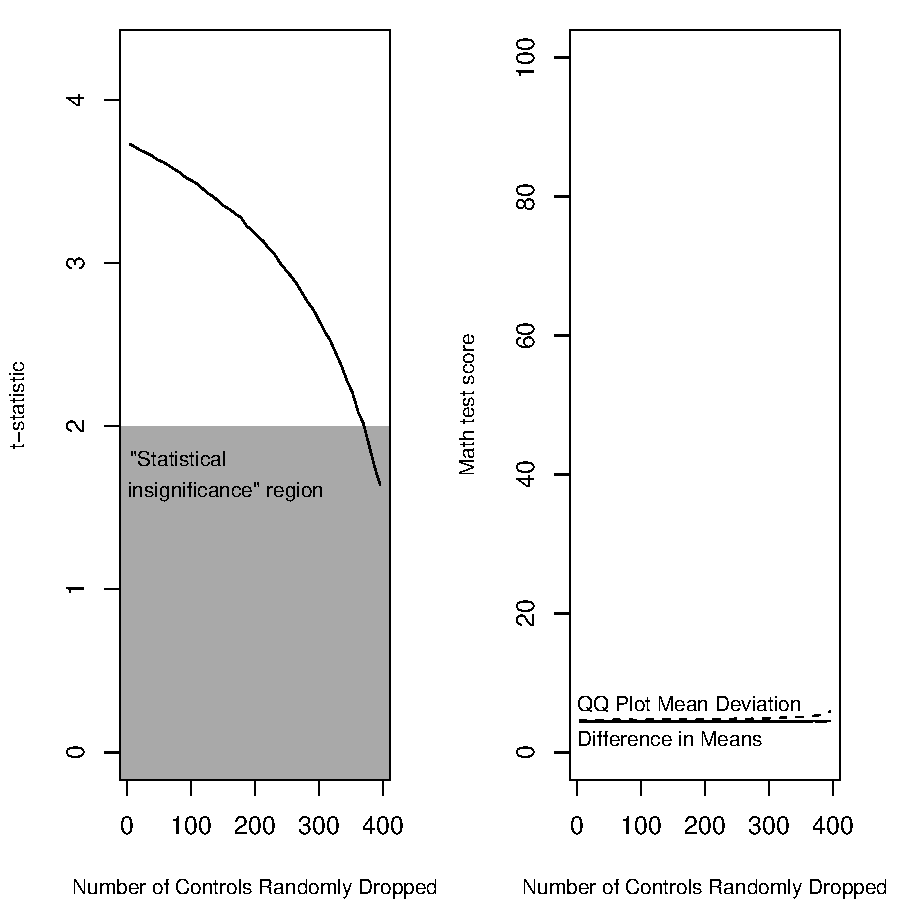
\includegraphics[height=4.5in]{figs/TStatPlotR0MATH}
  \caption{\em Dangers in relying on $t$-statistics as measure of balance.
    The lines in both graphs indicate the average value of a measure
    of balance when a given number of control units are randomly
    dropped from the data set (out of a total of 434).  With larger
    numbers of control units dropped (i.e., smaller numbers of control
    units in the resulting sample), the value of the $t$-statistic gets
    closer to 0, falsely indicating improvements in balance, even
    though true balance does not vary systematically across the data
    sets (and efficiency declines).  The difference in means and
    quantile-quantile plot mean deviation, given in the right graph,
    correctly indicate no change in bias as observations are randomly
    dropped.}
  \label{f:randrop}
\end{figure}

Second, the problem in Figure~\ref{f:randrop} can be seen by
recognizing that dropping observations can influence not only balance
but also statistical power, and unfortunately the $t$-test, like most
statistical tests, is a function of both.  The more observations
dropped, the less power the tests have to detect imbalance in observed
covariates.  Formally, let $n_{mt}$ and $n_{mc}$ be the sample sizes
for the matched treated and matched control groups, and define
$r_m=n_{mt}/n_m$ where $n_m=n_{mt}+n_{mc}$. Then, write the two sample
$t$-test statistic with unknown and unequal variances as
\begin{equation}
  \label{ttest} \frac{\sqrt{n_m}(\overline{X}_{mt}-\overline{X}_{mc})}
               {\sqrt{\frac{s^2_{mt}}{r_m} + \frac{s^2_{mc}}{1-r_m}}}
\end{equation}
where $\overline{X}_{mt}=\sum_{i=1}^{n_m} T_i X_i/n_{mt}$ and
$\overline{X}_{mc}=\sum_{i=1}^{n_m} (1-T_i)X_i/n_{mc}$ are the sample
means, and $s^2_{mt}=\sum_{i=1}^{n_m} T_i(X_i -
\overline{X}_{mt})^2/(n_{mt}-1)$ and $s^2_{mc}=\sum_{i=1}^{n_m}
(1-T_i)(X_i - \overline{X}_{mt})^2/(n_{mc}-1)$ represent the sample
variances of the matched treated and control groups, respectively.
Hence, the difference in sample means as a measure of balance is
distorted in the $t$-test by three factors: (1) the total number of
remaining observations $n_m$, (2) the ratio of remaining treated units
to the total number of remaining observations $r_m$, and (3) the
sample variance of $X$ for the remaining treated and control units,
$s_{mt}^2$ and $s_{mc}^2$.  Since the value of (this and other)
hypothesis tests are affected by factors other than balance, they
cannot even be counted on to be monotone functions of balance: The
$t$-test can indicate balance is getting better while the actual
balance is getting worse, staying the same, or improving.

Third, from a theoretical perspective, balance is a characteristic of
the sample, not some hypothetical population, and so, strictly
speaking, hypothesis tests are irrelevant in this context
\citep{HoImaKin06,Hansen06}.  Virtually all methods of adjustment
condition on the observed values of $X$, and so $X$ can be dropped in
these analyses only when Equation~\ref{balance} is satisfied in
sample, not in some population from which the data are hypothetically
or actually drawn.  For the same reason that randomized blocks or
paired matching are preferable to classical randomization in
experimental design --- that is, the imbalance in the variables that
defines the blocks can be set to zero in-sample, without having to
hope that the sample size is large enough for the advantages of
randomization to kick in \citep[see also][p.264]{GreLuSil04} ---
matching on all observed differences in $X$ is preferable whenever
feasible.  Indeed, in the best case, we would be able to match exactly
on all observed covariates, and afterwords randomize the assignment of
values to the treatment variable $T$.  That is, imbalance --- the
difference between $\tilde p(X\mid T=1)$ and $\tilde p(X\mid T=0)$ ---
should be minimized without limit where possible, so long as we are
not unduly compromising other goals in the process (such as
efficiency).

Finally, we offer a simple model that conveys why matching contains no
de minimus level, below which the level of imbalance is acceptable.
To see this, consider data generated by the classical regression
model, $E(Y\mid T,X)= \theta + T\beta + X\gamma$ \citep{Goldberger91}.
Then the regression of $Y$ on a constant and $T$ (without $X$) gives a
difference in means, the (conditional) bias of which as an estimate of
$\beta$ is $E(\hat\beta-\beta\mid T,X) = G\gamma$, where $G$ contains
vectors of coefficients from regressions of each of the variables in
$X$ on a constant and $T$.  Using matching to eliminate bias under
this simplified data generation process involves dropping or repeating
observations so that $G$ is as close to a matrix of zeros as possible.
But what happens to bias if $G$ is smaller than it was before matching
but still not zero?  The answer is that the bias is reduced, but
without knowledge of $\gamma$ --- which researchers eschew estimating
to avoid inadvertently introducing selection bias by choosing matching
solutions that stack the deck for their favored hypotheses --- it
could be that a nonzero portion of $G$, when multiplied by its
corresponding elements of $\gamma$, will generate arbitrarily large
bias.  This also shows that no measure of balance which is a function
of $X$ alone can be guaranteed to be a monotone function of bias
without special assumptions \citep{RubStu06}, and so proper measures
of imbalance should always be minimized without limit, subject to
efficiency constraints.  Thus, whether or not some hypothesis tests
indicate that $G$ is not significantly different from zero is
immaterial: The smaller $G$ is the better, either above or below the
$t$-test threshold of statistical significance, since $G$ (i.e.,
balance) is a characteristic of the observed data.  

An argument related to our last point has been made in the context of
randomized experiments, where researchers have shown that even small
(and statistically insignificant) differences in important (or what
they call in this literature ``prognostic'') covariates can result in
large differences in the results of the experiment
\citep{Altman85,Senn94,PocAssEno02}.  However, the problem we describe
in this section with power and stopping rules being a function of the
remaining sample size does not arise in randomized experiments.


\section{Appropriate Evaluation of Matching Solutions}

Balance should thus be checked by comparing the observed covariate
differences between the treated and control groups and the difference
should be minimized without limit.  A difference in means is a fine
way to start.  (Statisticians tend to standardize the mean differences
so the measure can be compared across different variables.  This is a
reasonable approach when simplification is necessary, but the
standardization also makes the variables invariant to the substantive
research question, and to priors about likely values of $\gamma$ or
the equivalent.) Other options include higher order moments than the
mean, nonparametric density plots, and propensity score summary
statistics \citep{AusMam06, Hansen04, Rubin01}. A more general
approach is quantile-quantile (or ``QQ'') plots that compare the
empirical distribution of two variables, although statistics based on
QQ plots can have higher variance.  In each case, the statistics
chosen to assess balance should be characteristics of the sample and
not some hypothetical population.  The graph on the right side of
Figure~\ref{f:randrop} plots for comparison the difference in means
and a QQ plot summary statistic, the average distance between the
empirical quantile distributions of the treated and control groups
calculated over the same samples as the left graph.\footnote{Formally,
  this measure can be defined as $\frac{1}{n} \sum_{i=1}^n
  |\widetilde{F}_{Xmt}^{-1}(i/n) - \widetilde{F}^{-1}_{Xmc}(i/n)|$
  where $\widetilde{F}_{Xmt}$ and $\widetilde{F}_{Xmc}$ are the
  empirical distribution functions of a covariate $X$ for the matched
  treated and matched control groups, respectively, and
  $n=\min(n_{mt},n_{mc})$.}  Unlike the $t$-test, the level of balance
does not change for either statistic as more units are randomly
dropped.  These statistics are by no means perfect, but they and many
others do not have the flaw we show hypothesis tests possess when used
as a stopping rule for assessing balance.  As is widely recognized, we
also ultimately need better ways of comparing two multidimensional
histograms, but these should be sample quantities, not hypothesis
tests.

Although these results indicate that future researchers should not use
hypothesis tests as a balance stopping rule, a reasonable question is
how to interpret the considerable volume of published literature that
did so without reporting better balance statistics.  One
interpretation would be that published tables which report small
p-values or large $t$-tests should cause readers to worry about
balance, whereas the reverse would not suggest any level of comfort
(which is analogous to the similarly narrow role for which they may be
useful in randomized experiments; \citealt{Senn94}).  Another way to
think about these hypothesis tests is as an analogy to the tests often
conducted in randomized experiments to check that the randomization
was done validly.  However, this analogy is imperfect because in a
randomized experiment researchers can be sure that any imbalance of
any size resulted by chance, while in an observational study,
imbalance could be due either to chance or to systematic differences
between the groups.  In addition, even this interpretation requires an
implicit reference to a hypothetical population, which is of
questionable direct relevance to the matched sample \citep{Cochran65}.
Best practice should be to minimize imbalance for all covariates,
using measures like those described above, and then to adjust
parametrically for any remaining differences
\citep{Rubin79,RosRub84a,HoImaKin06}.

\bigskip
\noindent {\bf formalization.} Suppose 
there are $n$ treated units and $n$ control units with a total of $2n$
units. Then, the {\it conditional} bias for estimating the average
treatment effect is given by,
\begin{eqnarray*}
  &    & {\rm Bias} \\
  & =  & \frac{1}{2n} \sum_{i=1}^{2n} E[Y_i(1) -
  Y_i(0) \mid X_i] - \left\{\frac{1}{n} \sum_{i \, \in \{T_i =1 \}}
  E[Y_i(1) \mid X_i] - \frac{1}{n} \sum_{i \, \in \{T_i =0 \}}
  E[Y_i(0) \mid X_i] \right\}, \\
  & = & \frac{1}{2n} \left\{ \sum_{i\,\in \{T = 0\}} E[Y_i(1) \mid
  X_i] - \sum_{i\,\in \{T = 1\}} E[Y_i(1)
  \mid X_i] + \sum_{i\,\in \{T = 0\}}
  E[Y_i(0) \mid X_i] - \sum_{i\,\in \{T = 1\}} E[Y_i(0) \mid X_i]\right\}, \\
  & = & \frac{1}{2} \left\{\int E[Y(1) \mid T = 0, X] d\widetilde{F}(X \mid T =
  0) - \int E[Y(1) \mid T = 1, X] d\widetilde{F}(X \mid T =
  1)\right\} \\
  &  &  + \frac{1}{2} \left\{ \int E[Y(0) \mid T = 0, X] d\widetilde{F}(X \mid T =
  0) - \int E[Y(0) \mid T = 1, X] d\widetilde{F}(X \mid T =
  1)\right\}, \\
  & = &  \frac{1}{2} \int E[Y(1) \mid T = 0, X] \,d[\widetilde{F}(X \mid T
  = 0) - \widetilde{F}(X \mid T = 1)] \\
   &  & + \frac{1}{2} \int\left\{ E[Y(1) \mid T = 0, X] - E[Y(1) \mid T = 1,
  X]\right\}\, d\widetilde{F}(X \mid T = 1)\\
  &  & + \frac{1}{2} \int E[Y(0) \mid T = 0, X] \,d[\widetilde{F}(X \mid T
  = 0) - \widetilde{F}(X \mid T = 1)] \\
   &  & + \frac{1}{2} \int\left\{ E[Y(0) \mid T = 0, X] - E[Y(0) \mid T = 1,
  X]\right\}\, d\widetilde{F}(X \mid T = 1),\\
  & = &  \frac{1}{2} \int E[Y(1) + Y(0) \mid T = 0, X]\,d[\widetilde{F}(X \mid T
  = 0) - \widetilde{F}(X \mid T = 1)] \\
   &  & + \frac{1}{2} \int\left\{ E[Y(1) + Y(0) \mid T = 0, X] -
  E[Y(1) + Y(0)\mid T = 1,
  X]\right\}\, d\widetilde{F}(X \mid T = 1).
\end{eqnarray*}
The randomization removes the second term, which is the bias due to
the violation of the ignorability assumption, but it does not remove
the first term, which is the bias due to the difference between two
empirical distributions. If you take the expectation of this bias over
the distribution of $X$, then clearly both terms are zero. This shows
that randomization leads to zero bias if there is no sampling bias.
Moreover, if $n$ goes to infinity, then $\widetilde{F}(X \mid T = t)$
converges almost surely to $F(X \mid T=t)$ for $t=0,1$
(Glivenko-Cantelli Theorem). And hence asymptotically, the bias of the
first term also goes away under randomization.

Now, let's assume the following structural model
\begin{eqnarray*}
  Y_i(1) & = & g_1(X_i) + U_{1i}, \\
  Y_i(0) & = & g_0(X_i) + U_{0i}
\end{eqnarray*}
where $X_i$ is observed while $(U_{i1}, U_{i0})$ is not.  In
econometrics, we say that {\it separability} between $X$ and $(U_0,
U_1)$ is assumed. Now, we write the discrepancy as follows,
\begin{eqnarray*}
  & & {\rm Discrepancy}  \\
  & =  & \frac{1}{2n} \sum_{i=1}^{2n} [Y_i(1) -
  Y_i(0)] - \left\{\frac{1}{n} \sum_{i \, \in \{T_i =1 \}}
  Y_i(1) - \frac{1}{n} \sum_{i \, \in \{T_i =0 \}}
  Y_i(0) \right\}, \\
  & = & \frac{1}{2n} \left\{ \sum_{i\,\in \{T = 0\}} Y_i(1) - 
    \sum_{i\,\in \{T = 1\}}  Y_i(1) + \sum_{i\,\in \{T = 0\}}
  Y_i(0) - \sum_{i\,\in \{T = 1\}} Y_i(0) \right\}, \\
  & = & \frac{1}{2} \int [g_1(X) + g_0(X)] \,d[\widetilde{F}(X \mid T
  = 0) - \widetilde{F}(X \mid T = 1)]  \\
  & & + \frac{1}{2} \int [U_1 + U_0] \,d[\widetilde{F}(U_0 \mid T = 0) - \widetilde{F}(U_0 \mid
  T = 1)]   
\end{eqnarray*}
We can partially relax the separability assumption by postulating the
model, $Y_i(t) = g_t(X_i, U_{ti})$ for $t=0,1$. In that case, we get
\begin{eqnarray*}
  {\rm Discrepancy} & = & \int [g_1(X, U_1) + g_0(X, U_0)]\, d[\widetilde{F}(X, U_1 \mid
  T = 1) - \widetilde{F}(X, U_0 \mid T = 0)] 
\end{eqnarray*}
Finally, note that
\begin{eqnarray*}
  E({\rm Discrepancy} \mid X_i) = {\rm Bias}.
\end{eqnarray*}

%\baselineskip=0.637\baselineskip 
\clearpage
\bibliographystyle{apsr}
\bibliography{gk,gkpubs} 
\end{document}
